% ---------------------------------------------------------------------------
% Temporal profile of the corpus and of the extracted events.
% % ---------------------------------------------------------------------------
% Temporal profile of the corpus and of the extracted events.
% % ---------------------------------------------------------------------------
% Temporal profile of the corpus and of the extracted events.
% % ---------------------------------------------------------------------------
% Temporal profile of the corpus and of the extracted events.
% \input{figures/fig_corpus_temporal} — expects graphicx and a full-width
% (two-column) float. Asset: fig_corpus_temporal.pdf, regenerated by
% figures/make_fig_corpus_temporal.py (data are inlined in that script).
% ---------------------------------------------------------------------------
\begin{figure*}[t]
  \centering
  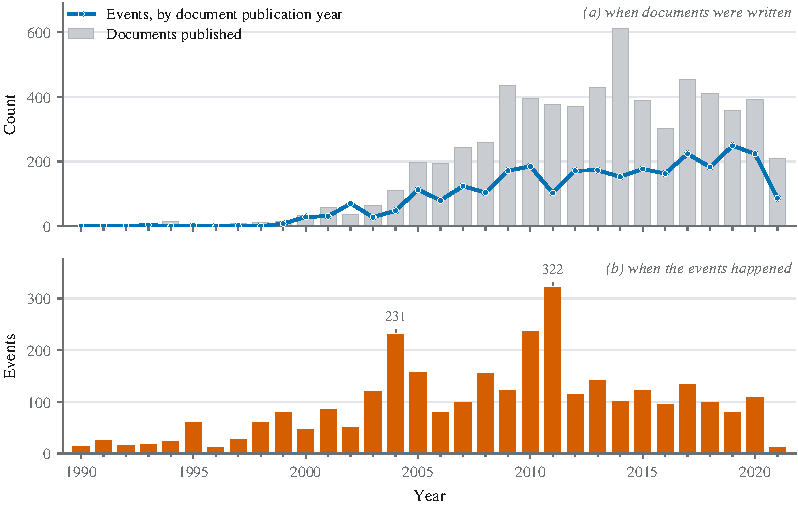
\includegraphics[width=\textwidth]{figures/fig_corpus_temporal}
  \caption{Temporal profile of the production run. (a) Documents by
  publication year (bars, $n=6{,}392$ of 10{,}000) and the verifiable events
  extracted from them, attributed to the document's publication year (line,
  $n=2{,}909$ of 3{,}572). (b) The same events placed at the date of the event
  itself ($n=3{,}046$ of 3{,}572). Document supply is a publication artifact
  --- it tracks UNDRR's reporting cycle and thins after 2021 --- whereas the
  event dates are spread across four decades and peak in years of
  large-footprint disasters. Axes are restricted to 1990--2021; off-axis are
  3{,}574 documents (662 events) with no parsable publication year, 87 events
  with no parsable event date, 2 documents from 1980--1989, 32 from
  2022--2025, and 439 events dated before 1990.}
  \label{fig:corpus-temporal}
\end{figure*}
 — expects graphicx and a full-width
% (two-column) float. Asset: fig_corpus_temporal.pdf, regenerated by
% figures/make_fig_corpus_temporal.py (data are inlined in that script).
% ---------------------------------------------------------------------------
\begin{figure*}[t]
  \centering
  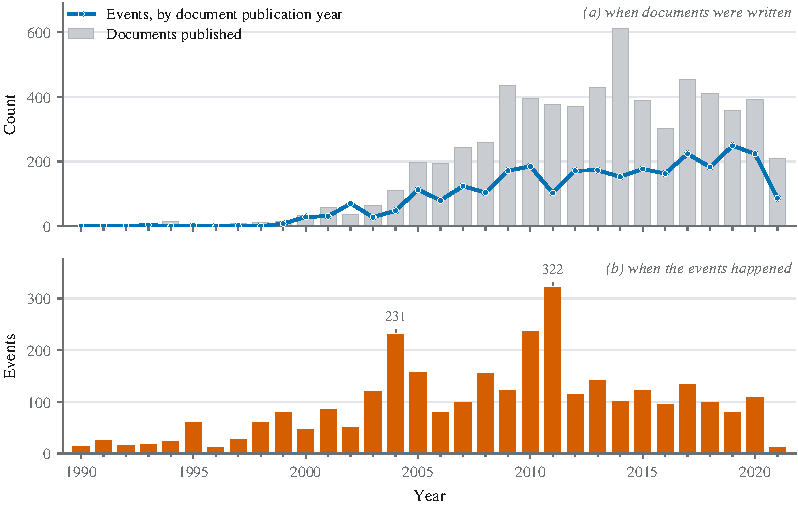
\includegraphics[width=\textwidth]{figures/fig_corpus_temporal}
  \caption{Temporal profile of the production run. (a) Documents by
  publication year (bars, $n=6{,}392$ of 10{,}000) and the verifiable events
  extracted from them, attributed to the document's publication year (line,
  $n=2{,}909$ of 3{,}572). (b) The same events placed at the date of the event
  itself ($n=3{,}046$ of 3{,}572). Document supply is a publication artifact
  --- it tracks UNDRR's reporting cycle and thins after 2021 --- whereas the
  event dates are spread across four decades and peak in years of
  large-footprint disasters. Axes are restricted to 1990--2021; off-axis are
  3{,}574 documents (662 events) with no parsable publication year, 87 events
  with no parsable event date, 2 documents from 1980--1989, 32 from
  2022--2025, and 439 events dated before 1990.}
  \label{fig:corpus-temporal}
\end{figure*}
 — expects graphicx and a full-width
% (two-column) float. Asset: fig_corpus_temporal.pdf, regenerated by
% figures/make_fig_corpus_temporal.py (data are inlined in that script).
% ---------------------------------------------------------------------------
\begin{figure*}[t]
  \centering
  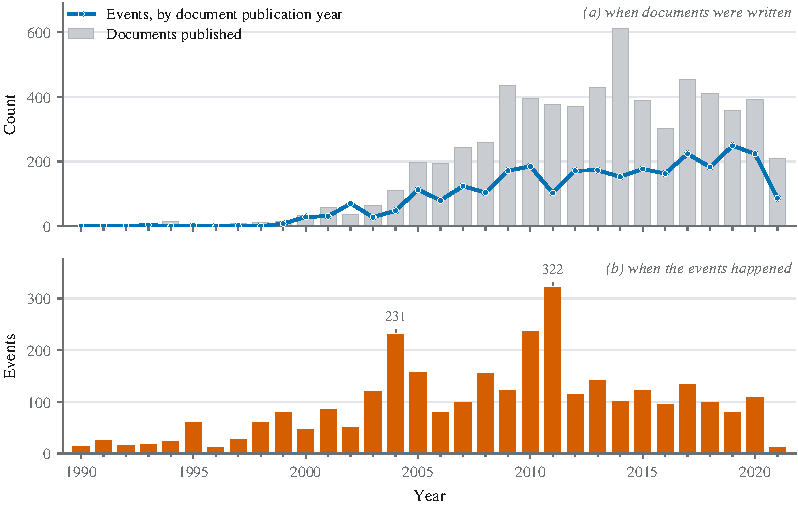
\includegraphics[width=\textwidth]{figures/fig_corpus_temporal}
  \caption{Temporal profile of the production run. (a) Documents by
  publication year (bars, $n=6{,}392$ of 10{,}000) and the verifiable events
  extracted from them, attributed to the document's publication year (line,
  $n=2{,}909$ of 3{,}572). (b) The same events placed at the date of the event
  itself ($n=3{,}046$ of 3{,}572). Document supply is a publication artifact
  --- it tracks UNDRR's reporting cycle and thins after 2021 --- whereas the
  event dates are spread across four decades and peak in years of
  large-footprint disasters. Axes are restricted to 1990--2021; off-axis are
  3{,}574 documents (662 events) with no parsable publication year, 87 events
  with no parsable event date, 2 documents from 1980--1989, 32 from
  2022--2025, and 439 events dated before 1990.}
  \label{fig:corpus-temporal}
\end{figure*}
 — expects graphicx and a full-width
% (two-column) float. Asset: fig_corpus_temporal.pdf, regenerated by
% figures/make_fig_corpus_temporal.py (data are inlined in that script).
% ---------------------------------------------------------------------------
\begin{figure*}[t]
  \centering
  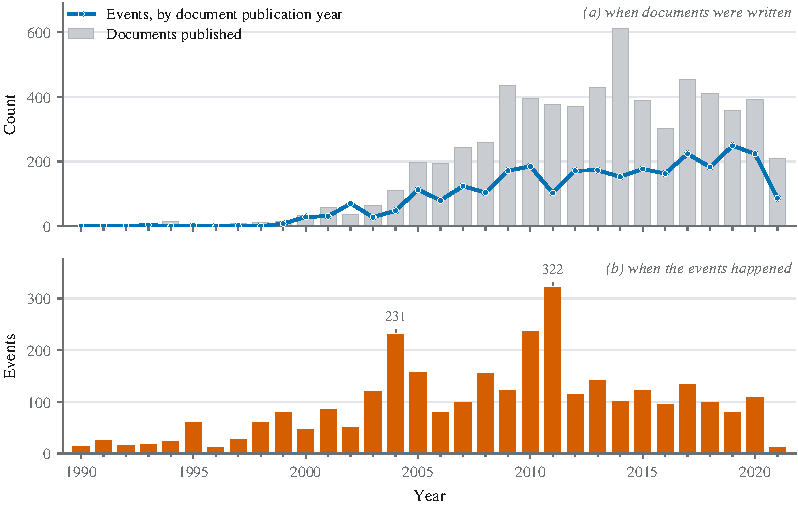
\includegraphics[width=\textwidth]{figures/fig_corpus_temporal}
  \caption{Temporal profile of the production run. (a) Documents by
  publication year (bars, $n=6{,}392$ of 10{,}000) and the verifiable events
  extracted from them, attributed to the document's publication year (line,
  $n=2{,}909$ of 3{,}572). (b) The same events placed at the date of the event
  itself ($n=3{,}046$ of 3{,}572). Document supply is a publication artifact
  --- it tracks UNDRR's reporting cycle and thins after 2021 --- whereas the
  event dates are spread across four decades and peak in years of
  large-footprint disasters. Axes are restricted to 1990--2021; off-axis are
  3{,}574 documents (662 events) with no parsable publication year, 87 events
  with no parsable event date, 2 documents from 1980--1989, 32 from
  2022--2025, and 439 events dated before 1990.}
  \label{fig:corpus-temporal}
\end{figure*}
